\chapter{Implementation}
Our main goal was to develop a high-performance algorithm. The implementation uses a distributed version of highly optimized kernel for central processing units (CPUs) and graphics processing units (GPUs), that runs efficiently on a cluster~\citep{Wittek20131165}. We extended this implementation to Hamiltonians that include external potential, to allow the simulation of a wider range of quantum systems. 

Particularly important for the purpose of high performance is the optimization of memory access patterns. Large amounts of data are stored in the main memory: the data needs to be sent to the processing unit. Nowadays, processing units are much faster in performing calculations than the ability of the main memories and the hardware bus to keep streaming data. So if the processing unit has to fetch data from the main memory, it would be limited by the bandwidth of the memory and the hardware bus. To avoid this problem, we exploit cache-aware computation that uses smaller and faster memories, dubbed caches~\citep{Handy}. 
Furthermore, a workload across a distributed memory system requires  communication between the nodes. To proceed to the next iteration, a node needs data of the previous iteration calculated by other nodes. The transfer of data in a network of nodes is even slower than the transfer from main memory to the processing unit. However, to a certain extent, communication between nodes and calculation in the processing unit can be done simultaneously. For the sake of efficiency, it is worth to overlap the two as much as possible.

For the purpose of developing reliable scientific software, we added unit testing to the implementation. In the development of complex software, it is important to test various parts of the code, to ensure its correctness. A program can be split into several units, each one having a defined use and an expected behaviour. Based on this, one can develop a test to exercise the unit and verify its exactness. We exploit unit testing using the library CppUnit~\citep{CPPUnit}. Moreover, we use double-precision floating point operations, to improve accuracy in the simulations.

Our approach was also to ensure that our implementation fits in with rapid prototyping
systems~\citep{SmithMF}. The program allows to the use of a command line interface, for the flexibility of the simulation. In addition, the function that performs the evolution is exposed as an application programming interface (API). We also developed wrappers to make the kernels accessible from the  high-level languages Python and MATLAB.

In this chapter, we describe the implementation of the evolution operator. There are two CPU kernels, one GPU kernel and a hybrid kernel that use both types of computational units. Before the kernel explanation, a short section introduces to the architecture of CPU and GPU memory hierarchy and gives some basic concepts of high performance programming. We end with the benchmark performed at the Barcelona Supercomputing Center.

%%%%%%%%%%%%%%%%%%%%%%%%%%%%%%%%%%%%%%%%%%%%%%%%%%%%%%%%%%%%%%%%%%%%%%%%%%%%%%%%%%%%%%
\section{Cache Optimization}
The gap between CPU speed and main memory performance is enormous. To alleviate this gap, computer architectures implement hierarchical memory structures. This approach allows to work around both the low main \textit{memory bandwidth} and the \textit{latency} of main memory accesses.
The memory bandwidth is a measure of the rate at which data can be read from or stored into the memory by a processor, and it is a crucial parameter that affects the performance of an algorithm. Furthermore, the memory latency plays an important role in the overall performance. The memory latency is the delay time between the moment a memory controller tells the memory module to access a particular memory location, and the moment these data become available on the module's output pins. These parameters characterized the velocity at which the memory can feed the processor. When the CPUs need to process a certain data, they request it from the memory, and wait for it to become available.
 
  The common structure of the hierarchy consists of a series of memories; the smaller they are, the closer they are to the CPUs; the cheaper they are, the further they are from the CPUs. Usually, at the top of the hierarchy there are the registers, memories integrated within the processor chip that can provide data with low latency and high bandwidth. Between the processor core and the main memory there are memories called \emph{cache memories} or \emph{caches}~\citep{Handy}. Finally, there is the main memory, that usually consist of large and slow RAM memories. During the execution of a program, some blocks of data are used more often than others, so the CPUs will work with this subset of data for most of the time. To get an efficient algorithm, the idea is to store frequently used blocks of data on fast memories: the more frequently the block is used, the higher in the hierarchy is the memory that stores it. 

Typically, the data residing within a smaller memory are also stored within the larger memory, so the levels of the memory hierarchy are subsets of one another. A common memory hierarchy is show in Fig.~\ref{fig:memory-hierarchy}.
\begin{figure}
   \centering
   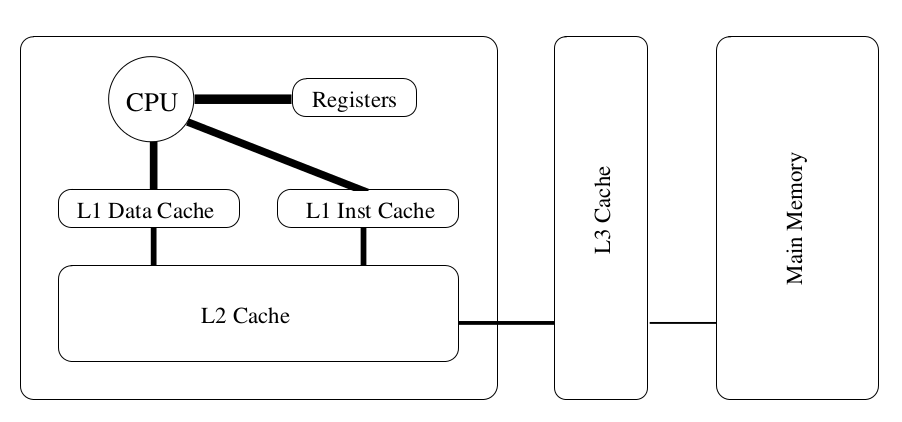
\includegraphics[width=10cm]{Figs/Memory_hierarchy.png}
   \caption{A Common memory hierarchy that present two on-chip L1 caches, on-chip L2 cache, and a third level of off-chip cache. The thickness of the interconnections illustrate the bandwidths between the memory hierarchy levels.} \label{fig:memory-hierarchy}
\end{figure} 

An efficient algorithm must consider the stages of the memory hierarchy. Unfortunately, compilers are not intended to introduce sophisticated cache-based transformations. Consequently, the optimization effort is left to the programmer. 

This aspect is particularly important when dealing with numerically intense codes, which occur in science and engineering disciplines, such as computational physics, mechanical engineering and computational fluid dynamics, just to mention some. These types of code are characterized by a large portion of floating-point operations, and small computational kernels. Thus, instruction cache misses do not significantly affect the execution performance. Much of the optimization effort concerns data access pattern. Indeed, due to data access latencies and memory bandwidth issues, it is not sufficient to optimize the number of arithmetic operation alone. Efficient codes in scientific computing must necessarily combine computationally optimal algorithms and memory hierarchy optimization.

%%%%%%%%%%%%%%%%%%%%%%%%%%%%%%%%%%%%%%%%%%%%%%%%%%%%%%%%%%%%%%%%%%%%%%%%%%%%%%%%%%%%
\subsection{Organization of Cache Architectures}
The common memory hierarchy presents a rather small number of registers on the chip, which has almost no memory latency. On the chip we can also find a small cache -- called \textit{level one (L1) cache} -- usually limited to 64~Kbyte, so that low latency and high bandwidth are assured. The latency of on-chip caches is commonly one or two CPUs cycles. The L1 cache is often split into two separate parts; one only keeps data, the other instructions. The second level memory (L2) is tipically placed on-chip as well and it is usually limited to 1~Mbyte. Due to the bigger size the  latency is around 5 to 10 cycles. Another cache level may be implemented off-chip if the L2 cache is on-chip. The L3 cache size may vary from 1~MByte to 16~MByte. They provide data with latency of about 10 to 20 cycles~\citep{Hennessy-Patterson}.

Data within the cache are stored in \textit{cache lines}. A cache line holds the contents of a contiguous block of main memory. We say that a cache hit occurs when the data requested by the processor is found in a cache line. If the data requested is not founded in the L1 cache, a cache miss occurs. In the latter case, the contents of the memory block containing the requested words are then fetched from a lower memory layer, for instance, from the L2 cache, and copied into a cache line. This operation typically implies another chunk data in L1 to be replaced by the requested one -- an operation that is very inefficient. Indeed, the replacement of a cache line takes more time than the CPU to read the same data directly from the main memory. For this reason, caches implement strategies to increase the rate of cache hits  over the cache misses. The optimal replacement strategy would be to replace the memory block which will not be accessed for the longest time. However, such strategy is impossible to implement since it requires information about future cache references. 
The most commonly used strategy is the \textit{least recently used}. It replaces the block which has not been accessed for the longest time interval.

%The most commonly used strategy is \textit{random} and \textit{least recently used}. The former randomly chooses a cache line to be replaced. The latter replaces the block which has not been accessed for the longest time interval. Less common strategies are \textit{least frequently used} and \textit{first in, first out}. The LFU replaces the memory block in the cache line which has least frequently been used, whereas the FIFO replaces the data which have been residing in cache for the longest time.
 

These strategy are based on the principle of locality references~\cite{Hennessy-Patterson}, which states that recently used data are very likely to be reused in the near future. Locality can be of two different type: temporal locality and spatial locality. A sequence of references exhibits temporal locality if recently accessed data are likely to be accessed again in the near future. A sequence of references manifest spatial locality if data located close together in address space tend to be referred close together in time.

%%%%%%%%%%%%%%%%%%%%%%%%%%%%%%%%%%%%%%%%%%%%%%%%%%%%%%%%%%%%%%%%%%%%%%%%%%%%%%%%%%%%%%
\subsection{Data Access Optimizations}
The most straightforward and simple approach to implement an algorithm, usually does not achieve the best execution performance. As we saw in the previous section, to reach this goal the programmer has to care about how the data movements are handled by the memory hierarchy and how the CPUs access data. In scientific computations, this typically implies the need to apply a transformation on the code, that change the order in which iterations in a loop nest are executed. Such transformations are part of data access optimizations techniques, where the goal is to improve temporal locality. We focus on a set of loop transformations that improve data locality for one level of the memory hierarchy: a cache.
\\

\noindent \textit{Loop Interchange}. This transformation reverses the order of two adjacent loops in a loop nest. This can be generalized to loop permutations where more than two loops are moved at once~\citep{Kennedy:2001:OCM:502981,Wolfe:1995:HPC:572937}.

A loop interchange can improve locality by reducing the \textit{stride} of an array-based computation. The stride is the distance of array elements in memory accessed within consecutive loop iterations. For instance, suppose we want to calculate the square norm of a vector (Algorithm~\ref{algo:loop-interchange}). Furthermore, suppose that the vector is stored in a 6 by 8 array in memory (Fig.~\ref{fig:interchanged-loop-nests}), in \textit{row major order}; that is, two array elements are stored adjacent in memory if their second indices are consecutive numbers. The code corresponding to the left part of Fig.~\ref{fig:interchanged-loop-nests}, accesses the array elements in a column-wise manner, so the stride is equal to 8. Consequently, the preloaded data in the cache line marked with grey color will not be reused if the array is too large to fit entirely in cache. The next element will be fetched from the main memory. Interchanging the loop nest allows the cache line to be reused, as the stride is now 1 (right part of Fig.~\ref{fig:interchanged-loop-nests}). \\
\begin{figure}
   \centering
   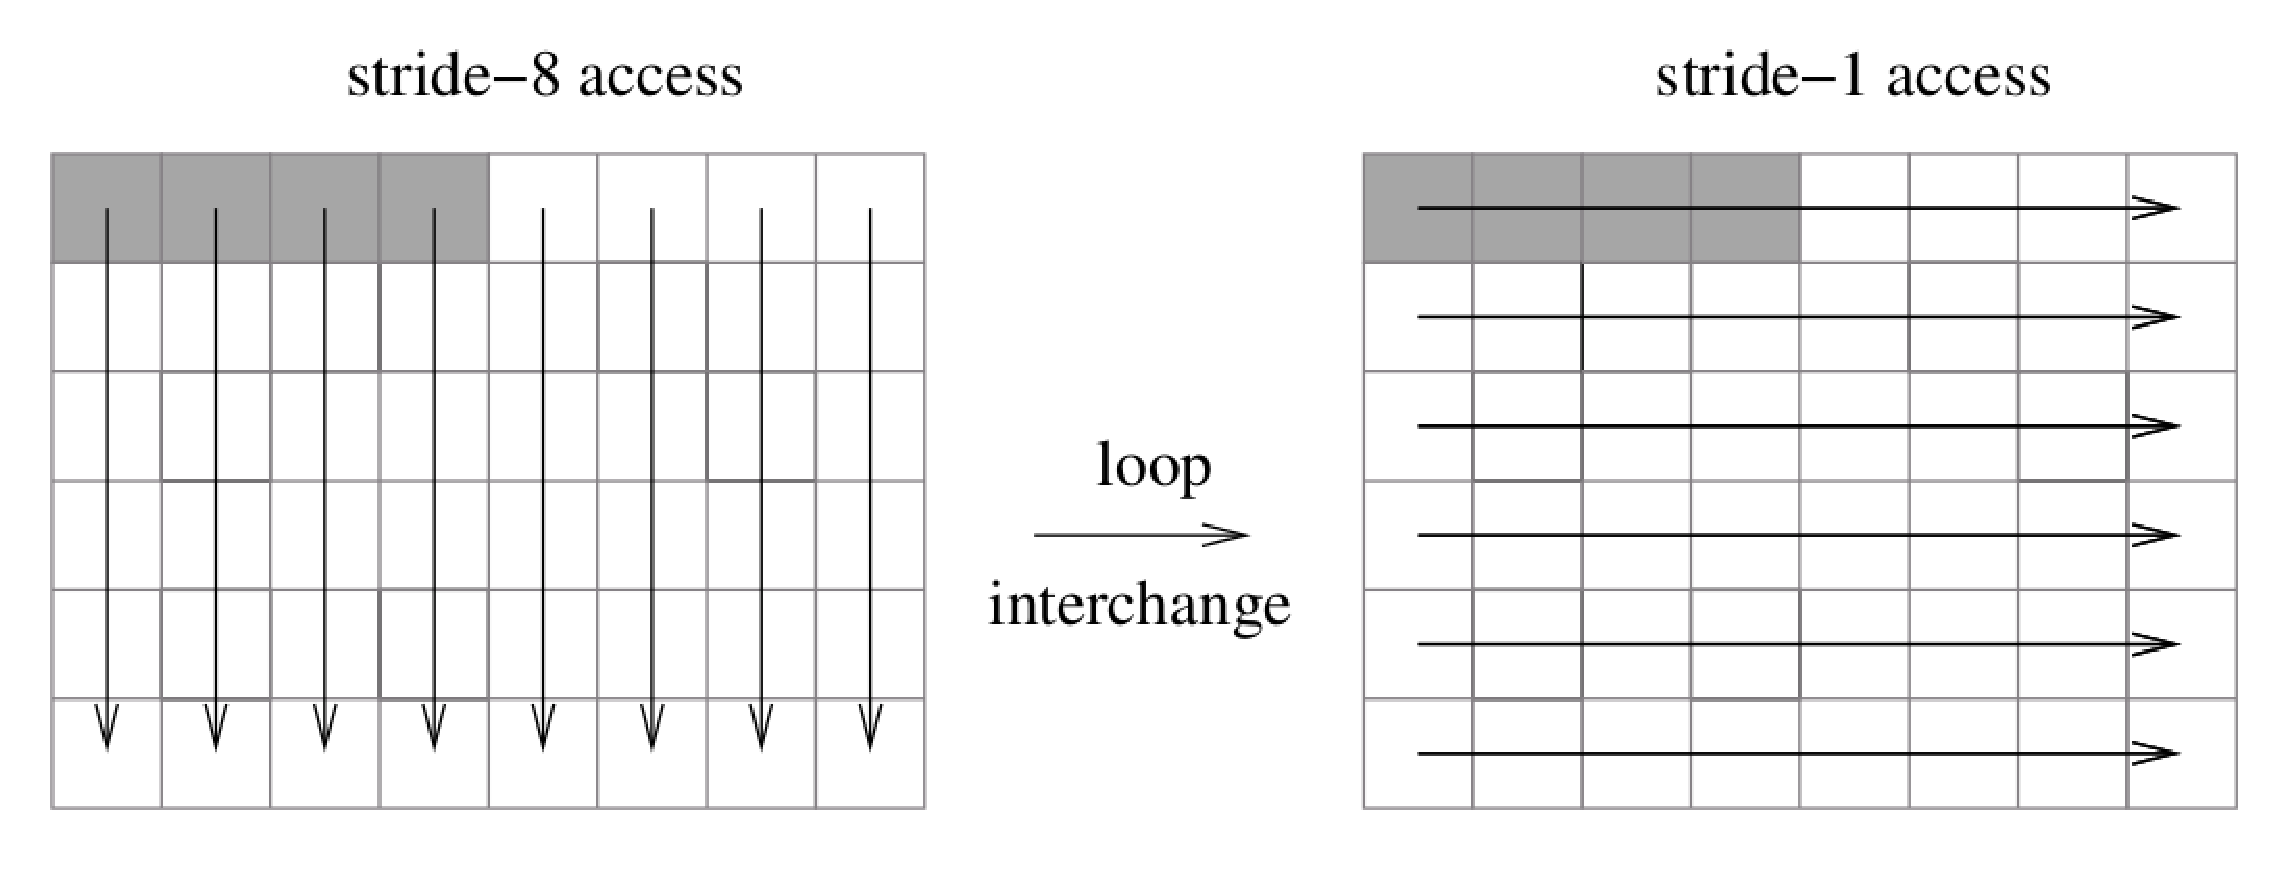
\includegraphics[width=10cm]{Figs/Interchanged_loop_nests.eps}
   \caption{Access pattern for interchenged loop nests in a (6,8) array.} \label{fig:interchanged-loop-nests}
\end{figure} 


\begin{algorithm}[t]
\SetAlgoLined
double $norm2$\;
double $a[n,n]$\;
//Original loop nest\;
\For{$j = 1$ \KwTo n }{
	\For{$i = 1$ \KwTo n }{
		$norm2 += a[i,j] \cdot a[i,j]$\;	
	}
}
\caption{Loop interchange} \label{algo:loop-interchange}
\end{algorithm}


\noindent \textit{Loop Fusion}. This transformation takes two adjacent loops that have the same iteration space traversal and combines their bodies into a single loop~\citep{Darte99onthe}.
When loop fusion can be applied -- when there are no instruction dependencies between the fused loops -- data locality may be improved. Assume that two consecutive loops perform global sweeps through an array as in the code shown in Algorithm~\ref{algo:loop-fusion},
and that the data are too large to fit entirely in the cache. When the first loop finishes, the elements of array \textit{b} are not completely loaded in cache, and the second loop will have to reload them from the main memory. If the two loops are combined with loop fusion only one global sweep through the array \textit{b} will be performed, resulting in fewer cache misses. \\
\begin{algorithm}[h]
//Original loop nest\;
\SetAlgoLined
\For{$i = 1$ \KwTo n }{
	$b[i] = a[i] + 1$\;
}
\For{$i = 1$ \KwTo n }{
	$c[i] = b[i] \cdot 3$\;
}
\caption{Loop fusion} \label{algo:loop-fusion}
\end{algorithm}

%%%%%%%%%%%%%%%%%%%%%%%%%%%%%%%%%%%%%%%%%%%%%%%%%%%%%%%%%%%%%%%%%%%%%%%%%%%%%%%%%%%%
\section{CPU Kernels}
The code implements two CPU kernels: both are  cache optimized, but one is further optimized to use the SSE instruction set of the CPU. In this section we explain the CPU kernels in a single thread scenario and the cache optimization strategy adopted.

%%%%%%%%%%%%%%%%%%%%%%%%%%%%%%%%%%%%%%%%%%%%%%%%%%%%%%%%%%%%%%%%%%%%%%%%%%%%%%%%%%%%
\subsection{Matrix Updating Scheme}
The initial wave function of the system $\psi_{i,j}(0)$ is stored in two arrays in row major order, one for the real part and one for the imaginary part. The evolved wave function $\psi_{i,j}(t)$ is calculated dividing the time in small time intervals of length $\Delta t$. To have an accurate simulation, $\Delta t$ must satisfy the inequality $\Delta t \ll \frac{m \Delta L^2}{\hbar}$, where $m$ is the particle mass and $\Delta L$ is the distance between two consecutive locations in the mesh. Indeed if we exploit the Taylor expansion of the evolution operator
\begin{equation}
\exp \left( \frac{\imath}{\hbar}H\Delta t \right) = 1 + \frac{\imath}{\hbar}H\Delta t + O(\Delta t^2),
\end{equation} 
we have $1 \gg \frac{\Delta t}{\hbar}\| H \| $. Suppose that the leading term in the Hamiltonian is the kinetic term, hence the second-order derivative approximation (Eq.~\eqref{eq:second-order-derivative}) leads to $1 \gg \frac{\hbar}{m \Delta L^2} \Delta t$.

In the second-order Trotter--Suzuki approximation, the $\psi_{i,j}(\Delta t)$ is the result of nine matrix-vector products. From Eq.~\eqref{eq:second-TS-evo-operator} and Eq.~\eqref{eq:1approxTS}, we have
\begin{align} \label{eq:single-iteration}
\psi(\Delta t) = \mathrm{e}^{\imath \frac{\alpha}{2} \hat{A}_y} \mathrm{e}^{\imath \frac{\alpha}{2} \hat{A}_x}   \mathrm{e}^{\imath \frac{\alpha}{2} \hat{B}_y} \mathrm{e}^{\imath \frac{\alpha}{2} \hat{B}_x}  \mathrm{e}^{-\frac{\imath \Delta t}{\hbar}\hat{V}} \mathrm{e}^{\imath \frac{\alpha}{2} \hat{B}_x} \mathrm{e}^{\imath \frac{\alpha}{2} \hat{B}_y} \mathrm{e}^{\imath \frac{\alpha}{2} \hat{A}_x} \mathrm{e}^{\imath \frac{\alpha}{2} \hat{A}_y} \psi(0)
\end{align}
where $\alpha = \frac{\hbar \Delta t}{2m\Delta L^2}$. Note that we discarded the phase changing factor $\mathrm{e}^{-\frac{\imath \Delta t \hbar}{m \Delta L^2} I}$ present in Eq.~\eqref{eq:1approxTS}. The exponential of the potential is diagonal and it is straightforward to implement: it is sufficient to multiply each element of the vector $\psi_{i,j}$ for the proper value (i.e. $\bra{i,j} \mathrm{e}^{-\frac{\imath t}{\hbar} \hat{V}} \ket{i,j}$). The matrix elements $\bra{i,j} \mathrm{e}^{-\frac{\imath t}{\hbar} \hat{V}} \ket{i,j}$ are calculated before the beginning of the kernel, and is stored on two real matrices in the main memory. With regards to the other exponential operators, the matrix vector multiplication can be decomposed in a series of linear combinations of couples of two neighbouring sites in the mesh. This can be easily understood from the form of $A$ and $B$ operators (Eq.~\eqref{eq:A-form} and Eq.~\eqref{eq:B-form}) that lead to Eq.~\eqref{eq:expA} and Eq.~\eqref{eq:expB}. Consider the couple $\psi_{i,j}$ and $\psi_{i,j+1}$, when $j$ is even, $\mathrm{e}^{\imath \frac{\alpha}{2} A_y}$ acts so that
\begin{align} \label{eq:single-coupling-operation}
\hat{\psi}_{i,j} = & \cos\left(\frac{\alpha}{2}\right) \psi_{i,j} + \imath \sin\left(\frac{\alpha}{2}\right) \psi_{i,j+1} \nonumber \\ 
\hat{\psi}_{i,j+1} = & \imath\sin\left(\frac{\alpha}{2}\right) \psi_{i,j} + \cos\left(\frac{\alpha}{2}\right) \psi_{i,j+1} 
\end{align}
In this operation, the sites $(i,j)$ and $(i,j+1)$ in the arrays are updated. We schematically represent this operation by mean of the diagram in Fig.~\ref{fig:scheme-single-iteration}.
\begin{figure}
   \centering
   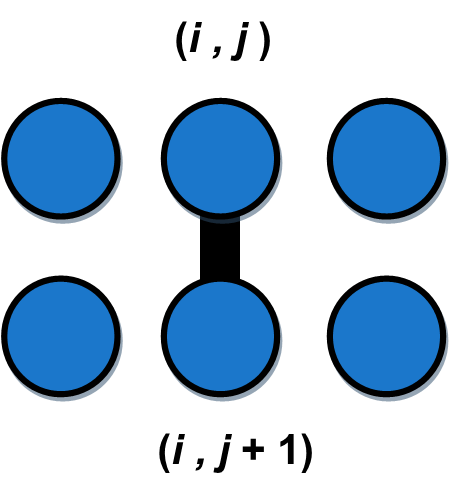
\includegraphics[width=2.5cm]{Figs/Single_couple.png}
   \caption{Single coupling operation.} \label{fig:scheme-single-iteration}
\end{figure}
Note that we do not need to store the exponential operator matrices $\mathrm{e}^{\imath \frac{\alpha}{2} A}$ and $\mathrm{e}^{\imath \frac{\alpha}{2} B}$. It is sufficient to store only two values: $ \cos\left(\frac{\alpha}{2}\right)$ and $\sin\left(\frac{\alpha}{2}\right)$.

Following this scheme, Eq.~\eqref{eq:single-iteration} can be schematized as in Fig.~\ref{fig:scheme-iteration}. The single time evolution is divided in nine computational steps corresponding to the matrix vector multiplications. Furthermore, the operations are independent from one another, so that sites in each computational step can be updated in place.

Regarding the imaginary time evolution, Eq.~\eqref{eq:single-coupling-operation} changes into:
\begin{align} \label{eq:single-coupling-operation-imag}
\hat{\psi}_{i,j} = & \cosh\left(\frac{\alpha}{2}\right) \psi_{i,j} + \sinh\left(\frac{\alpha}{2}\right) \psi_{i,j+1} \nonumber \\ 
\hat{\psi}_{i,j+1} = & \sinh\left(\frac{\alpha}{2}\right) \psi_{i,j} + \cosh\left(\frac{\alpha}{2}\right) \psi_{i,j+1} 
\end{align}
\begin{figure} 
   \centering
   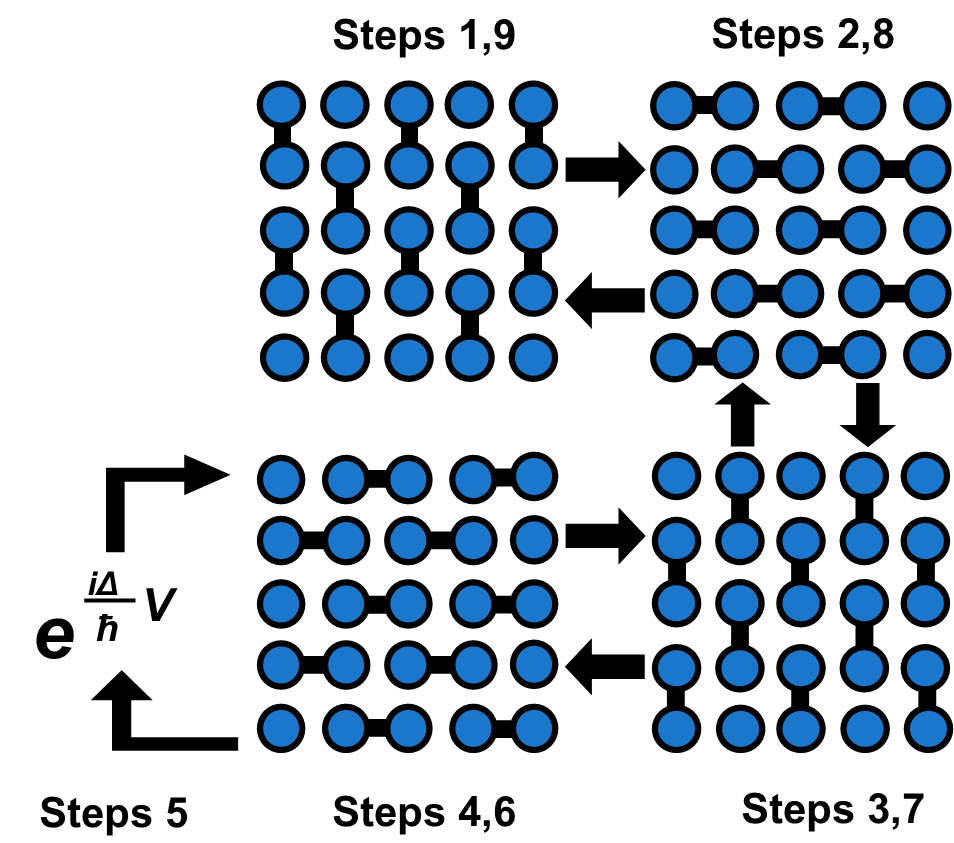
\includegraphics[width=8cm]{Figs/Single_time_step_evolution.png}
   \caption{Single time step evolution scheme for the second order Trotter--Suzuki.} \label{fig:scheme-iteration}
\end{figure}

%%%%%%%%%%%%%%%%%%%%%%%%%%%%%%%%%%%%%%%%%%%%%%%%%%%%%%%%%%%%%%%%%%%%%%%%%%%%%%%%%%%%
\subsection{Cache-aware Implementation}
A naive approach to implement the scheme in Fig.~\ref{fig:scheme-iteration} is by performing each computational step in a single pass over the entire array of sites. This performs efficiently as long as the array of sites fits in the cache, so that the CPU fetches the data directly from the cache. However, for large system sizes, data need to be fetched from the main memory, resulting in a drop in performance~\citep{bederian2011boosting}. 

Cache optimization can be achieved dividing the array of sites in blocks that fit in the cache and performing a single time step evolution for each one of them, separately. This raises the problem of data dependency. Suppose that a block has been read to the cache and evolved a number of steps. We cannot write the results back to the same array in the main memory, from where the block was read, as blocks adjacent to it still need some values on the boundary between the blocks for their own evolution. This is fixed through double buffering, allocating two arrays in the main memory instead of one and going back and forth between the two, reading from one and writing to the other.

Besides, to perform some computational steps on a block, we need the sites surrounding the block to be present in the cache as well, otherwise the sites on the edge of the block will not be valid. This is because each site needs their four neighbours to complete a single time step evolution. As we try to perform more computational steps on a block, the amount of nodes external to the block increases. These nodes generate a \textit{halo} around a block that must also be read into the cache and updated, but that at later steps become invalid because their own halos are not present. The minimum value of the halo thickness for a single time step evolution is of four sites, since there are four computational steps that couple sites for each direction.

In a non distributed version of the kernels a single CPU performs the time step evolutions as schematized in Fig.~\ref{fig:scheme-iteration}. Blocks of the array in the main memory, with their own halo, are written in the cache memory. A single time step evolution of the block is performed, writing the results back to the cache. The halo is discarded, while the block is written to the second buffer in the main memory (Fig.~\ref{fig:CPU-cache-optimization}). The multiple step strategy, combined with the tunable block size that depends on the hardware's cache size, puts the algorithm in the family of cache-aware stencil computations~\cite{kamil2006implicit}.
\begin{figure}
   \centering
   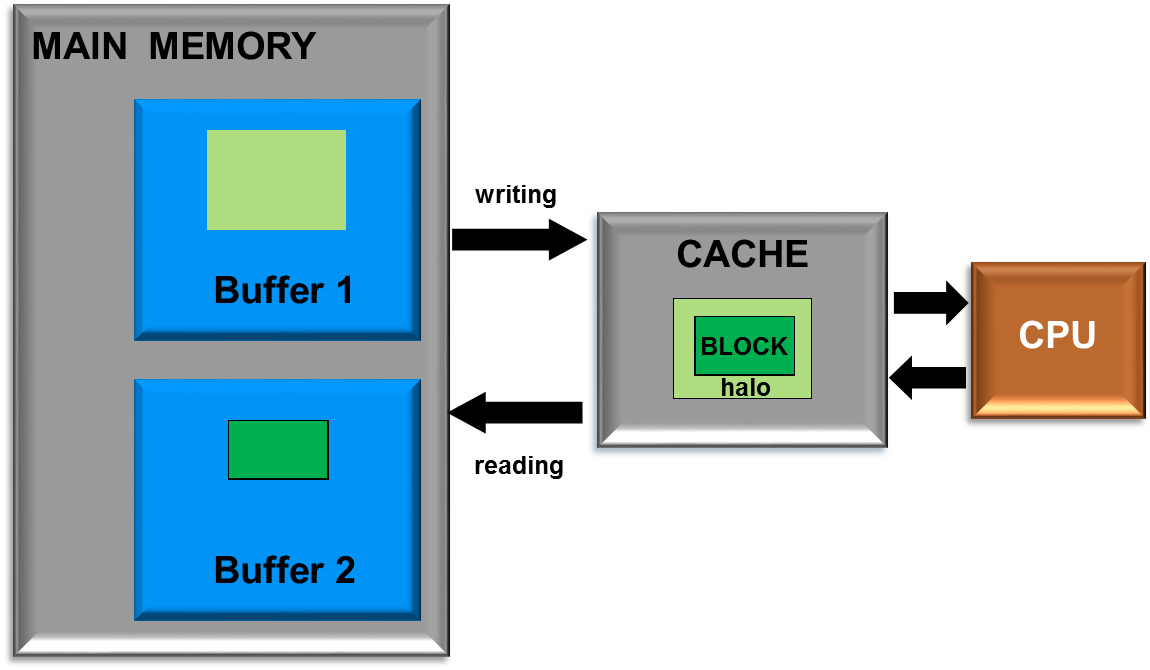
\includegraphics[width=10cm]{Figs/CPU-cache_optimization.png}
   \caption{Scheme of the CPU cache optimization. A time step evolution is performed, writing blocks of the first array into the cache.} \label{fig:CPU-cache-optimization}
\end{figure}

%%%%%%%%%%%%%%%%%%%%%%%%%%%%%%%%%%%%%%%%%%%%%%%%%%%%%%%%%%%%%%%%%%%%%%%%%%%%%%%%%%%%%
\section{GPU Kernel}
As the time step evolution is composed by simple and high parallelizable instructions, an implementation that runs on a GPU gains a high speed-up compare to a CPU kernel. Indeed, GPUs achieve a much high peak performances in certain parallel workloads compared to CPUs, as illustrated in Fig.~\ref{fig:CPU-GPU-computational-power}. This motivated the development of a GPU kernel. In this section, we outline the differences between the CPU and GPU architectures, describing the features of the latter. A description of the non-distributed version of GPU kernel follows.
\begin{figure}
   \centering
   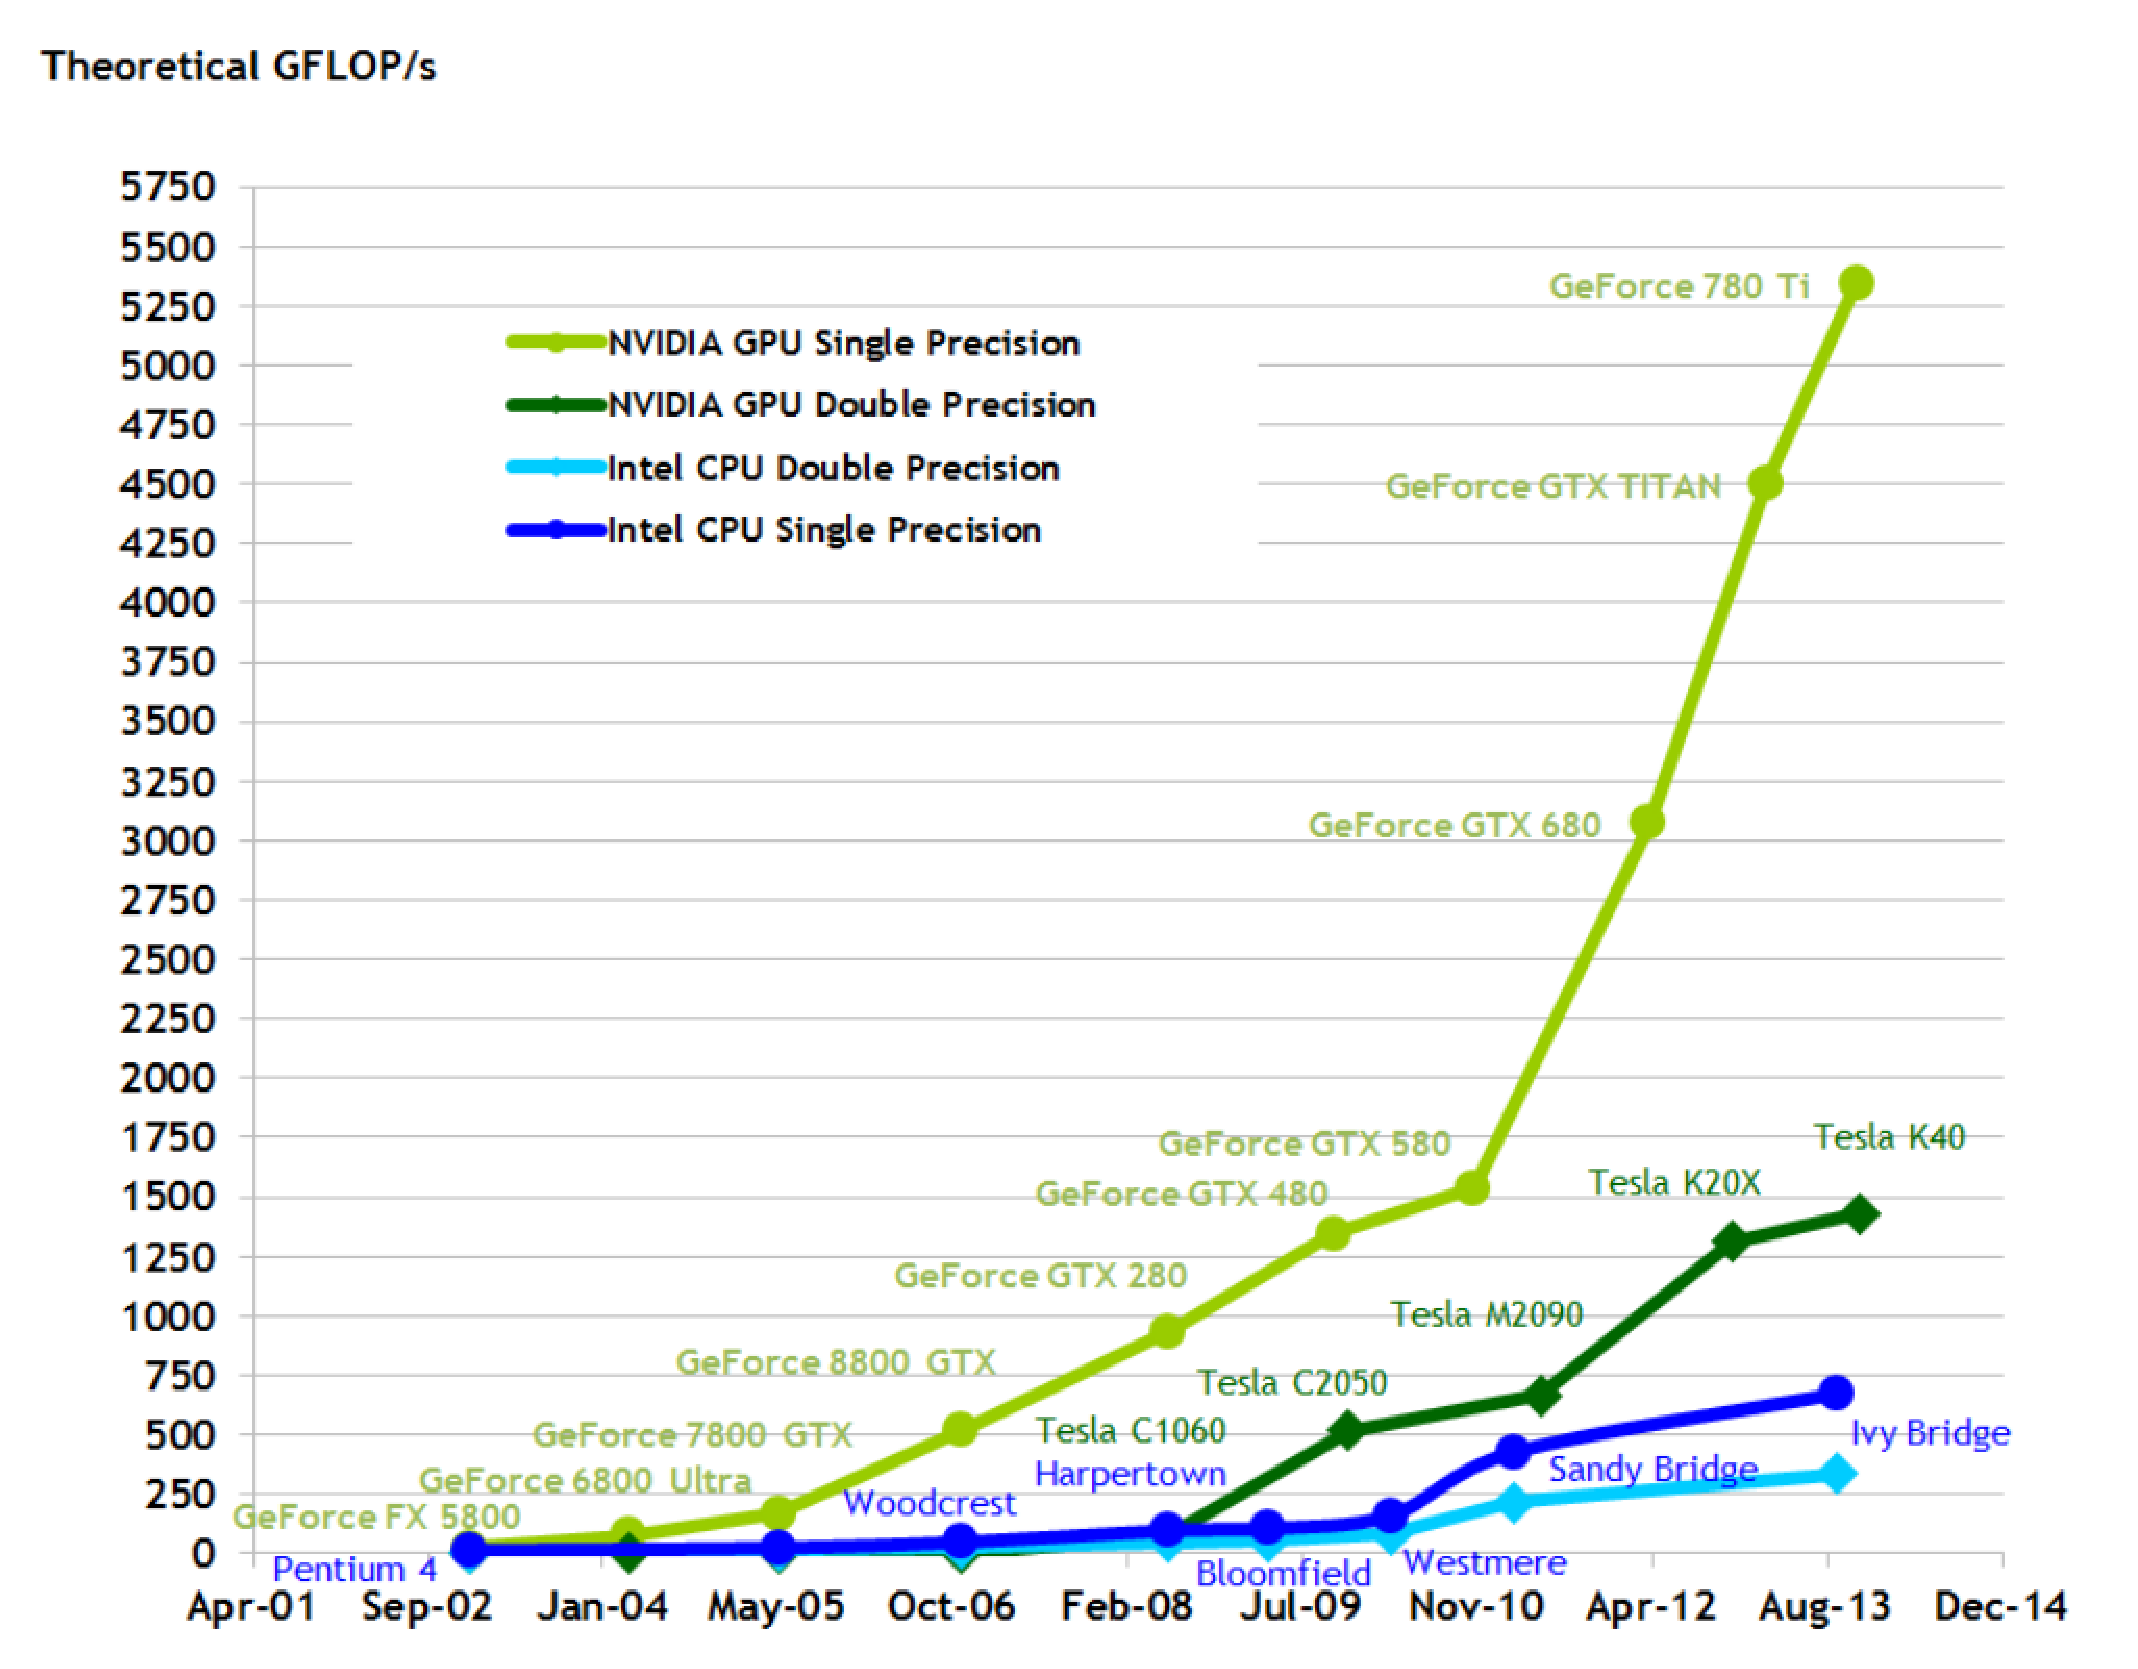
\includegraphics[width=10cm]{Figs/CPU-GPU_computational_power.eps}
   \caption{Floating-point operations per second for the CPU and GPU.} \label{fig:CPU-GPU-computational-power}
\end{figure}

%%%%%%%%%%%%%%%%%%%%%%%%%%%%%%%%%%%%%%%%%%%%%%%%%%%%%%%%%%%%%%%%%%%%%%%%%%%%%%%%%%%%%
\subsection{GPU Structure}
The reason behind the discrepancy in floating-point capability between the CPU and the GPU is that the GPU is specialized for compute-intense, highly parallel computation and therefore designed such that more transistors are devoted to data processing rather than data caching and flow control. Indeed, a GPU is well-suited to address problems that can be expressed as data-parallel computations, where the same calculation is executed on many data elements in parallel. Consequently,  a sophisticated flow control mechanism is unnecessary. Furthermore, because the program is executed on many data elements and has high arithmetic intensity, the memory access latency can be hidden with calculations instead of large data caches.

GPUs adopt the so-called \textit{single instruction, multiple thread} architecture as parallel execution model. Data elements are processed by sequences of parallel instructions called \textit{threads}. The NVIDIA GPU architecture is built around a scalable array of multithreaded \textit{Streaming Multiprocessors}. Threads are managed, created, scheduled and executed by streaming multiprocessors in groups of 32 parallel threads called \textit{warps}. Individual threads composing a warp start together at the same program address, but they have their own instruction address counter and register state and are therefore free to branch and execute independently. When a multiprocessor is given one or more thread blocks to execute, it partitions them into warps and each warp gets scheduled by a warp scheduler for execution. 

A warp executes one common instruction at a time, so full efficiency is realized when all 32 threads of a warp agree on their execution path. If threads of a warp diverge via a data-dependent conditional branch, the warp serially executes each branch path taken, disabling threads that are not on that path, and when all paths complete, the threads converge back to the same execution path (Fig.~\ref{fig:warp-instruction}). Branch divergence occurs only within a warp; different warps execute independently regardless of whether they are executing common or disjoint code paths. Consequently, the execution achieve better performance avoiding threads in a warp to branch.
\begin{figure}
   \centering
   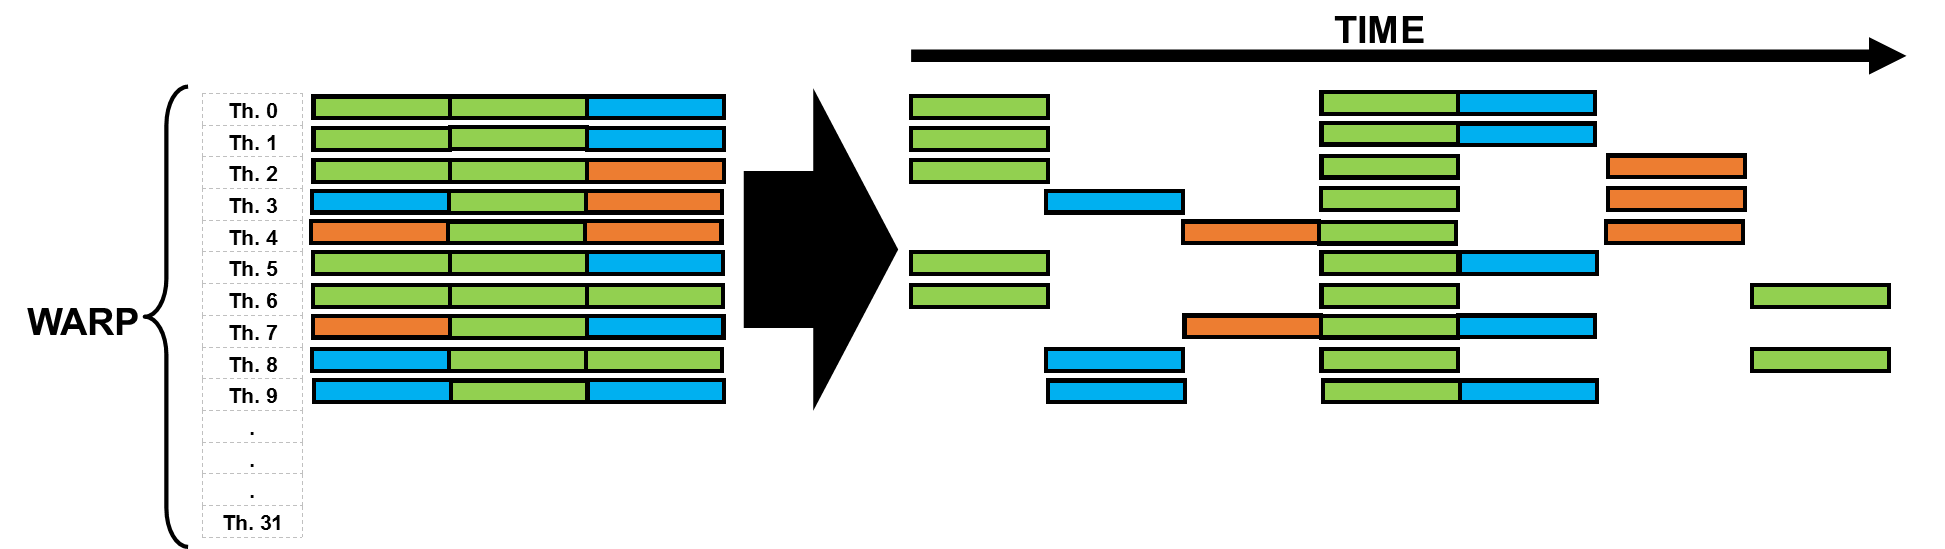
\includegraphics[width=14cm]{Figs/Warp_instruction.png}
   \caption{Instance of a warp execution. The left part of the graph illustrates the instructions to be performed by each thread. Each thread execute three instructions; instructions with the same color are identical. The right part of the graph illustrates how the instructions are executed by the threads within a warp. Threads, that execute the same instruction, perform the instruction at the same time. Different instructions are performed on different times. In this example threads are not in the same execution path -- there are at least three different paths -- resulting in a inefficient time performance.} \label{fig:warp-instruction}
\end{figure}

GPU are easily programmed using CUDA (Compute Unified Device Architecture) an extension of high-level programming language C. CUDA extends C by allowing the programmer to define C functions (kernels) that are executed $N$ times in parallel by N different \textit{CUDA threads}. Each thread is associated to a 3-component vector, so that they can be organized in a 1D, 2D or 3D structure. Groups of threads are collected in \textit{thread blocks}, whose size is dictated by the programmer. However, there is a limit to the number of threads per block, since all threads of a block are expected to reside on the same processor core and must share the limited memory resources of that core. Blocks are organized into a \textit{grid} of thread blocks, which can be one, two or three dimensional.

A GPU's memory is organized in a hierarchy, as it is also the case for the CPU (Fig.~\ref{fig:GPU-memory-hierarchy}). Closest to the processors there are fast and small registers, in which each thread store a private local memory space. On the next level in the hierarchy, there are \textit{shared memories}. Each thread block has access to a memory space stored on shared memories, which is visible to all the threads of the block. The last level consist in the global memory, accessible by all the threads.
\begin{figure}
   \centering
   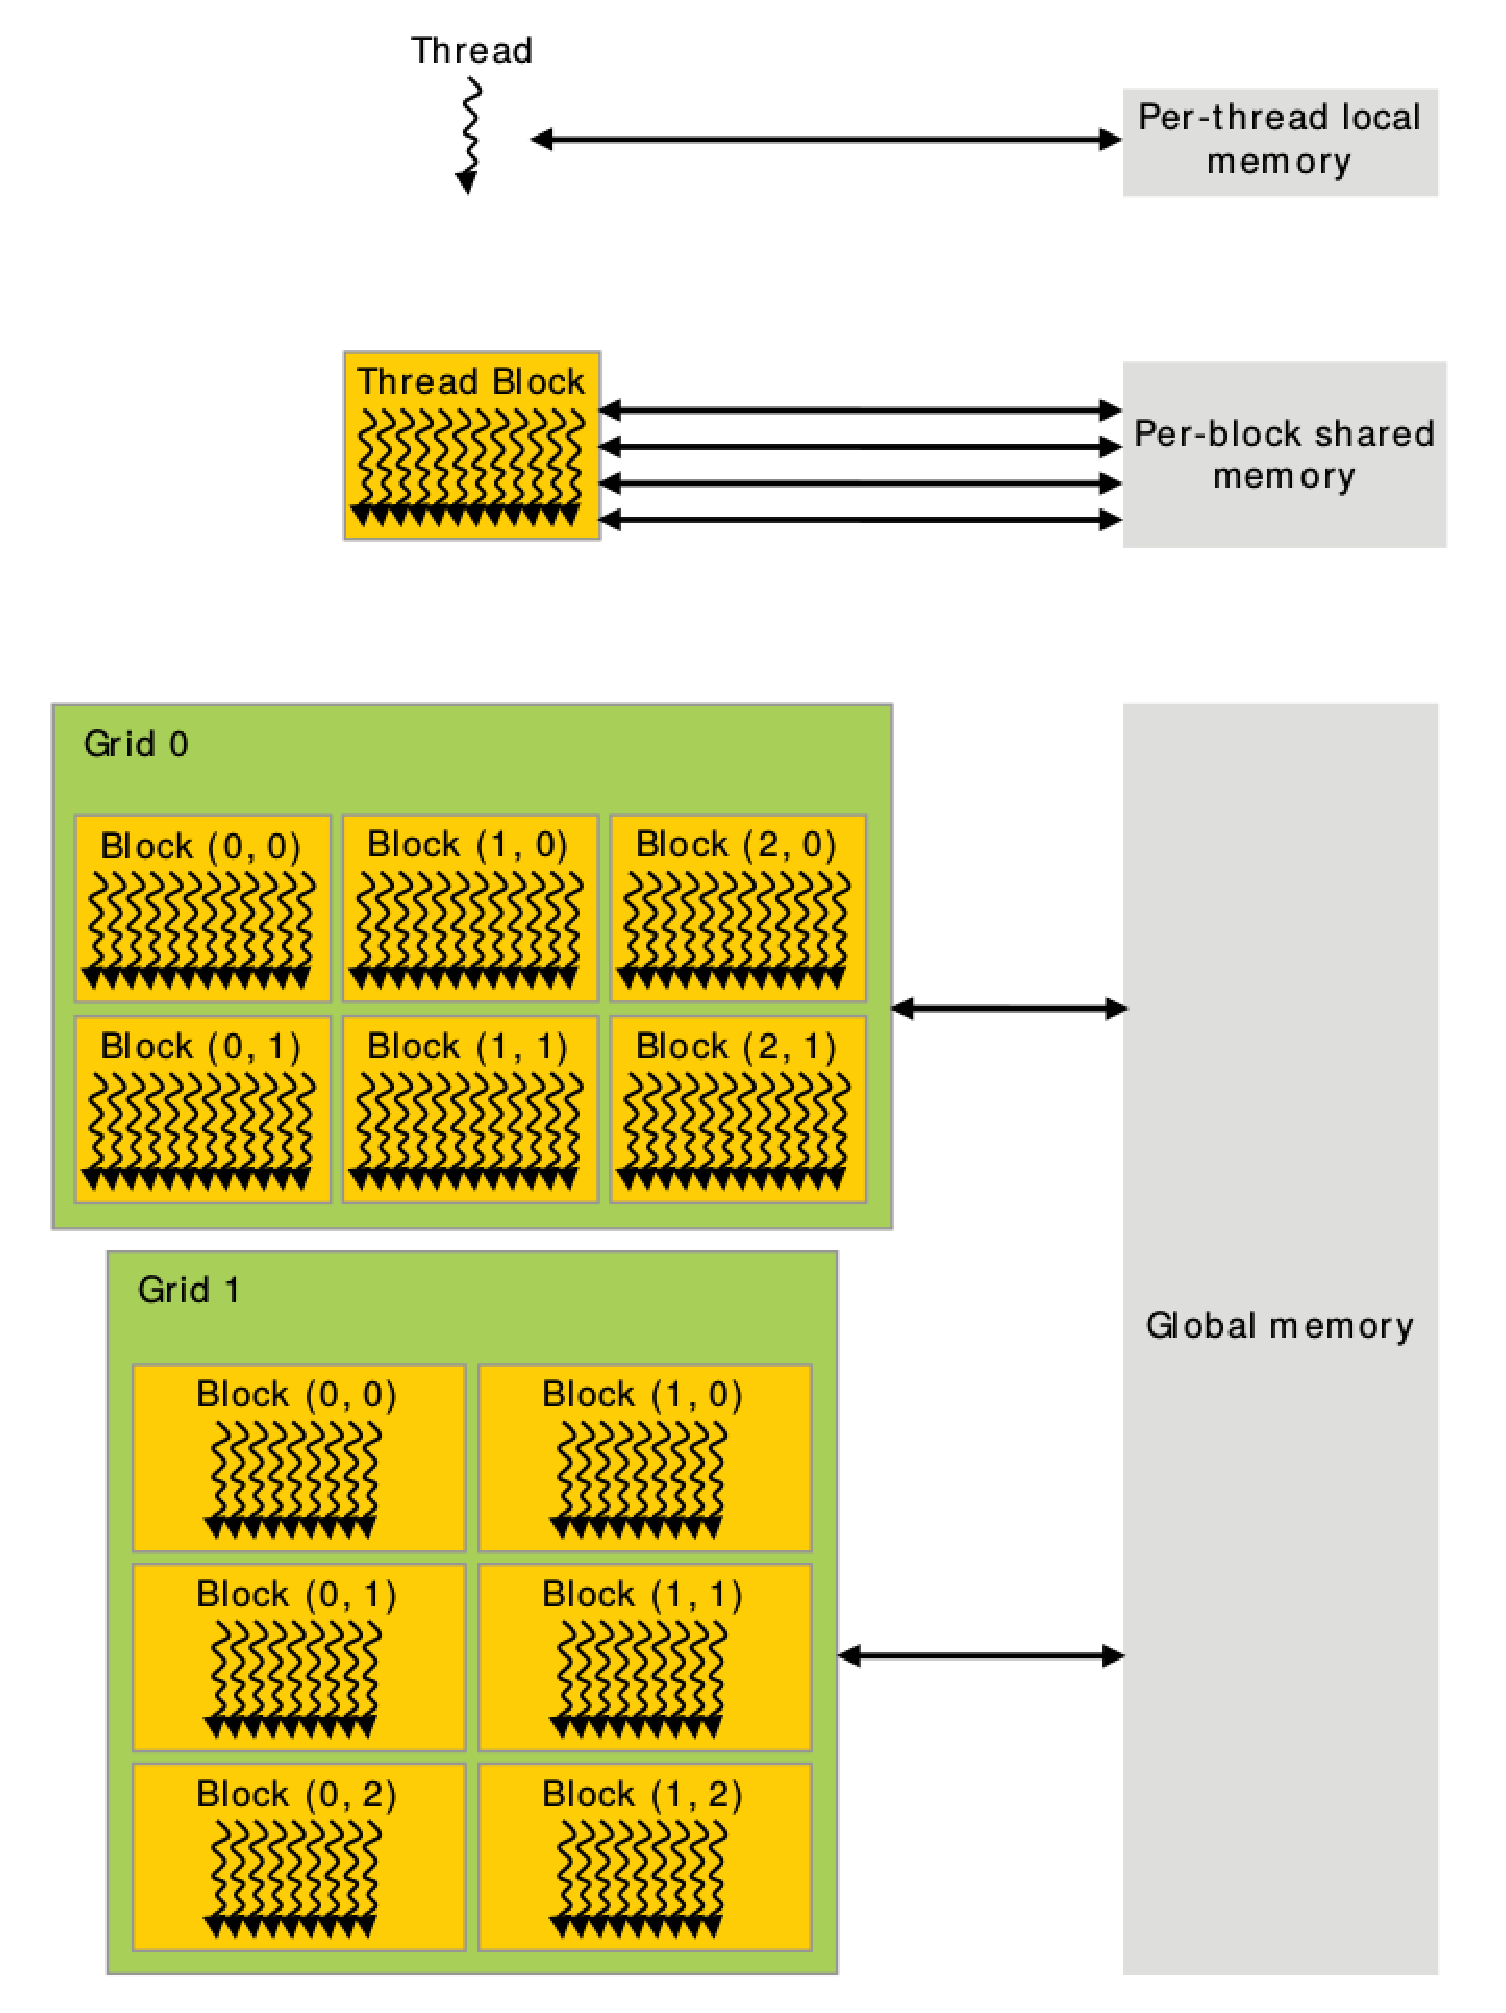
\includegraphics[width=10cm]{Figs/GPU_memory_hierarchy.eps}
   \caption{GPU memory hierarchy.} \label{fig:GPU-memory-hierarchy}
\end{figure}

%In the CUDA programming model, the GPU is regarded as a physically separate \textit{device} that operates as a coprocessor to the \textit{host} -- the CPU -- running the compiled C program. This is the case when the kernel executes on a GPU, while the rest of the C program executes on a CPU. Moreover, host and device communicate to share data. In particular, the host can allocate and deallocate space on the device global memory, as well as transfer data between host main memory and device global memory.
%write about heterogeneous programming?

%%%%%%%%%%%%%%%%%%%%%%%%%%%%%%%%%%%%%%%%%%%%%%%%%%%%%%%%%%%%%%%%%%%%%%%%%%%%%%%%%%%%%
\subsection{GPU Implementation}
The GPU kernel implements the same time step evolution as the CPU kernel (Fig.~\ref{fig:scheme-iteration}). In analogy with the CPU kernel, the  GPU kernel divides the array of sites in blocks, which are written in the shared memories of the multiprocessors, along with their own halo. This strategy benefits from the higher bandwidth of the shared memories, as it happens for the CPU cache.~Double buffering is required for data dependency; two arrays in the global memory are allocated, one for reading and one for writing the results. Contrary to what happens for the CPU kernels, blocks are executed in parallel, reducing the time of the execution. 

The time step evolution is performed using half number of threads as there are sites in the shared memory. In particular, each thread executes a single coupling operation. Data is partitioned so that each thread process couples of neighbours sites. This is done by arranging the threads in a checkerboard pattern; each thread allocates in its local memory the element corresponding to its position in the checkerboard, keeping it during all the single time step evolution execution. Then, it updates the value of this element and the one in its neighbour in the shared memory, which is determined by the computational step that is currently executed. The single coupling operations are executed in parallel by the threads, but the computational steps are processed in a serialized manner, due to data dependency. Hence, after each computational step there is a synchronization barrier. 
%schematic fig

%%%%%%%%%%%%%%%%%%%%%%%%%%%%%%%%%%%%%%%%%%%%%%%%%%%%%%%%%%%%%%%%%%%%%%%%%%%%%%%%%%%%%
\section{Hybrid Kernel}
During the execution of the GPU kernel, the host's CPU is idle while waiting for the GPU to complete the calculations. This CPU time could be used to perform part of the evolution of the state. Furthermore, GPU have less memory than CPU, limiting the size of the quantum system for which the evolution is computed. A hybrid kernel that uses both CPU and GPU address these two issues.

The algorithm calculates the maximum amount of the array sites that can be computed on the GPU. Then an internal area of the array site, with the appropriate size, is sent to the GPU to be calculated. Since CPU and GPU are in charge of evolving different area of the array sites, GPU requires a halo surrounding the internal area while the CPU needs the halo that correspond to the sites at the edge of the internal area. A single time step evolution is performed, using the CPU and GPU kernels described above for the corresponding areas. After that, the internal halos must be updated by performing a communication between CPU and GPU. The GPU receives the halo from the corresponding part of the mesh evolved by the CPU -- for the CPU is the other way around. 

The kernel also uses a directive-driven parallelism to utilize the power of a multicore system, relying on OpenMP~\citep{dagum1998openmp}. In the CUDA programming model, each GPU is associated to a single host, which is a single CPU core, hence, in a system with a multicore CPU and a single GPU, only one single CPU core would be used. For this purpose, the CPU kernel is slightly adjusted to use OpenMP, so that the blocks which divide the CPU mesh are processed in parallel using more than one CPU core.

%%%%%%%%%%%%%%%%%%%%%%%%%%%%%%%%%%%%%%%%%%%%%%%%%%%%%%%%%%%%%%%%%%%%%%%%%%%%%%%%%%%%%
\section{Distributing the Workload Across a Cluster}
The code is designed to run in a distributed multi-node system. The whole mesh is partitioned in blocks called tiles. Each node processes a tile plus its halo. After a single time step evolution the halos between the tiles have to be sent across the nodes. The communication is implemented using MPI~\citep{snir1998mpi}. Using a two-dimensional grid of nodes, a tile contains elements of halos belonging to a total of eight other tiles: left, right, top, and bottom neighbours, and also the four diagonal neighbours. To minimize the number of communication requests, a wave pattern is used in the communication: left and right neighbours receive the halo first. This halo has the height of the inner cells of the tile. Then the horizontal halos are sent to the top and bottom neighbours – the width is the full tile width. In this way the appropriate corner elements are propagated to the diagonal neighbours.

The communication is performed asynchronously: each halo is sent at the same time. However, there is a communication barrier between the left-right and top-bottom halo exchange due to data dependency. To achieve better performance, the approach is to overlap communication and evolution as much as possible, evolving the halo first and starting the communication simultaneously to the evolution of the rest of the tile. 

The CPU kernels evolve blocks of the tile at its edge, corresponding to the halos. Then the asynchronous left-right halo exchange and the evolution of the inner part of the tile initiates. Once finished the evolution of the inner part, there is the left-right halo exchange barrier. Consequently, the asynchronous top-bottom halo exchange starts and the top-bottom barrier ensure that it finish before swapping the buffers and continuing with the next time step. In this case, the halo exchange cannot be efficiently overlapped with computation, since, after the time step evolution is finished, there is a communication overhead while the vertical halos are exchanged.

As regard the GPU kernel, the communication is performed from the host memory. This increases the complexity, as asynchronous memory copies from the device and to the device have to be performed. To work with such transfer efficiently, the kernel implements \textit{streams}. A GPU stream is basically a queue of tasks for the GPU to perform: kernel execution, and memory copies from and to the device. Tasks in two different streams can overlap with each other, while tasks on the same stream are performed sequentially. When the host queues a task into a GPU stream, it does not have to wait for the task to be completed by the GPU before continuing with the rest of the algorithm. Two streams are implemented in the kernel: queueing the halo computation and the memory copies between host and device in stream one, and the computation of the inner part of the tile in stream two.

The host starts queueing the evolution of the blocks at the edge of the tile, corresponding with the halo, and the halo copy from device to host in stream one. While the GPU is running the first stream, the host queues the evolution of the rest of the blocks in the second stream. Once the GPU finishes the tasks in the first stream the halo can be exchanged between the nodes, using the wave pattern described above. With this approach, the communication of all halos is efficiently overlapped with the blocks calculation -- the task in the second stream. When the halo communication is completed, the host queues the copy of the halos received to the device memory in the first stream. Once the GPU finishes the tasks in each streams, the buffers in the global memories are swapped and the kernel starts over.

%We say that certain GPUs allow device-to-device transfer without involving the host memory, and some configurations also allow similar transfers between GPUs located in different hosts. We assumed that GPU-GPU communication would always involve the host memory.

%We use one process per GPU, and single-node execution with multiple GPUs is possible.

The hybrid kernel uses only one stream to queue the tasks for the GPU. The host launch the GPU kernel for the corresponding sites on the internal area of the tile. After that the host -- CPU -- proceeds to calculate the halo and start the halo exchange. Once the halo exchange is initiated, the sites not in the halo and not on the GPU are evolved by the CPU. Finally, finished the halo exchange, it exchange the internal halo between the part of the tile associated with the GPU and the rest of the matrix.

%%%%%%%%%%%%%%%%%%%%%%%%%%%%%%%%%%%%%%%%%%%%%%%%%%%%%%%%%%%%%%%%%%%%%%%%%
\section{Benchmarks}
To study the scaling pattern of the execution time as the number of nodes vary, we ran benchmarks on the Minotauro cluster at the Barcelona Supercomputing Center. The Minotauro cluster is comprised of 126 compute nodes, where each node has two Intel Xeon E5649 six-core processors with 12~MB of cache memory, clocked at 2.53~GHz, running a Linux operating system with 24~GB of RAM memory. Every node is equipped with two NVIDIA M2090 graphic cards, each one with 512 CUDA cores and 6~GB of GDDR5 memory. The MPI communication across the nodes is through an Infiniband Network. 

The benchmarks ran ten iterations on increasing cluster sizes, using an initial state in a square domain of different lenghts $L$: 4096, 8192, 16384. The dimensions were chosen so as to fill the device memory on cluster sizes 1, 4 and 16 nodes. GPUs have a better performance when the load is higher, whereas CPUs are less sensitive to the load. For this reason, choosing a matrix dimension that fit the GPUs, we get a fair comparison with respect to the CPU kernels due to their insensitivity to the load. Furthermore, this configuration shows how the overall performance decays as the cluster size increases. The times of execution are shown in Table~\ref{tab:bench-time} and they are also plotted in Figs.~\ref{plot:bench-4096}-\ref{plot:bench-16384}.
The results show only the time taken in the main loop of the evolution, as each kernel takes different amounts of time for initialization.

The CPU kernels show an almost linear scaling: as the cluster size is doubled, the execution time is halved. The communication overhead increases with the cluster size, so eventually the advantage of SSE optimization vanishes with large clusters.

The GPU kernel shows a different scaling pattern. When the device memory is loaded to at least 50\%, the scaling is close to linear, as in the case of CPU kernels. For lower load, the scaling is less efficient, until the execution time of individual GPUs remains almost constant so the curve flattens out. There is little benefit to gain by this kernel in large clusters with a low resolution of the mesh.

The hybrid kernel shows a pattern similar to the GPU. In this configuration, where the matrix size fit the GPU memory, the execution time is slightly longer. The real advantage is in cases where the device memory is insufficient. In such cases, the speedup can be  close to a factor of 2 compared to the CPU kernels.

\begin{table}
\centering
\begin{tabular}{*{13}{l}}
\hline
Nodes & \multicolumn{4}{l}{Matrix size: $4096$} & \multicolumn{4}{l}{Matrix size: $8192$} \\
 & CPU & SSE & CUDA & Hybrid & CPU & SSE & CUDA & Hybrid \\
\hline
1 & 5.30 & 5.01 & 0.65 & 0.84 &  & & & \\
2 & 2.68 & 2.55 & 0.38 & 0.53 &  & & 1.14 & 1.56 \\
4 & 1.37 & 1.29 & 0.29 & 0.34 & 5.37 & 5.10 & 0.66 & 0.85 \\
8 & 0.68 & 0.65 & 0.20 & 0.27 & 2.69 & 2.57 & 0.46 & 0.59 \\
16& 0.36 & 0.34 & 0.17 & 0.21 & 1.35 & 1.29 & 0.32 & 0.40 \\
32& 0.20 & 0.18 & 0.18 & 0.22 & 0.72 & 0.68 & 0.27 & 0.34 \\
\hline
\end{tabular}

\vspace*{0.5 cm}

\begin{tabular}{*{13}{l}}
\hline
Nodes & \multicolumn{4}{l}{Matrix size: $16384$} \\
 & CPU & SSE & CUDA & Hybrid \\
\hline
4 &  &  & 2.27 & 3.00 \\
8 & 1.07 &  & 1.24 & 1.68 \\
16& 0.53 & 5.04 & 0.74 & 0.90 \\
32& 0.28 & 2.66 & 0.49 & 0.68 \\
\hline
\end{tabular} \caption{Execution time.} \label{tab:bench-time}
\end{table}

\begin{figure}
   \centering
   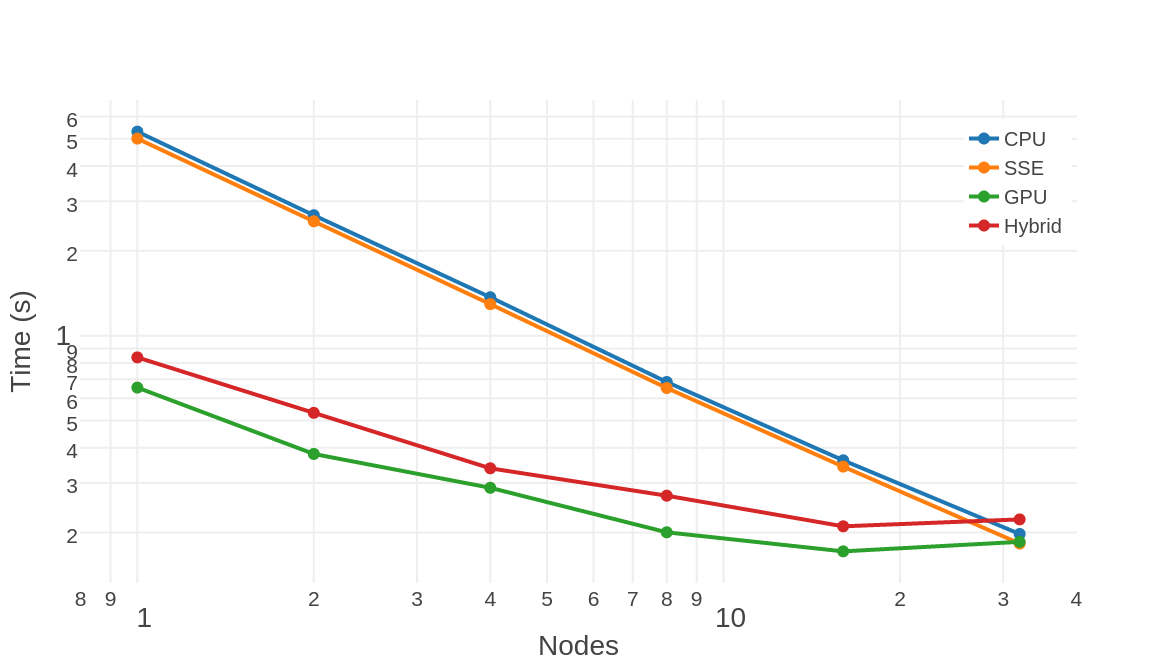
\includegraphics[width=11cm]{Plots/4096.png}
   \caption{Execution time for linear system size: 4096.} \label{plot:bench-4096}

   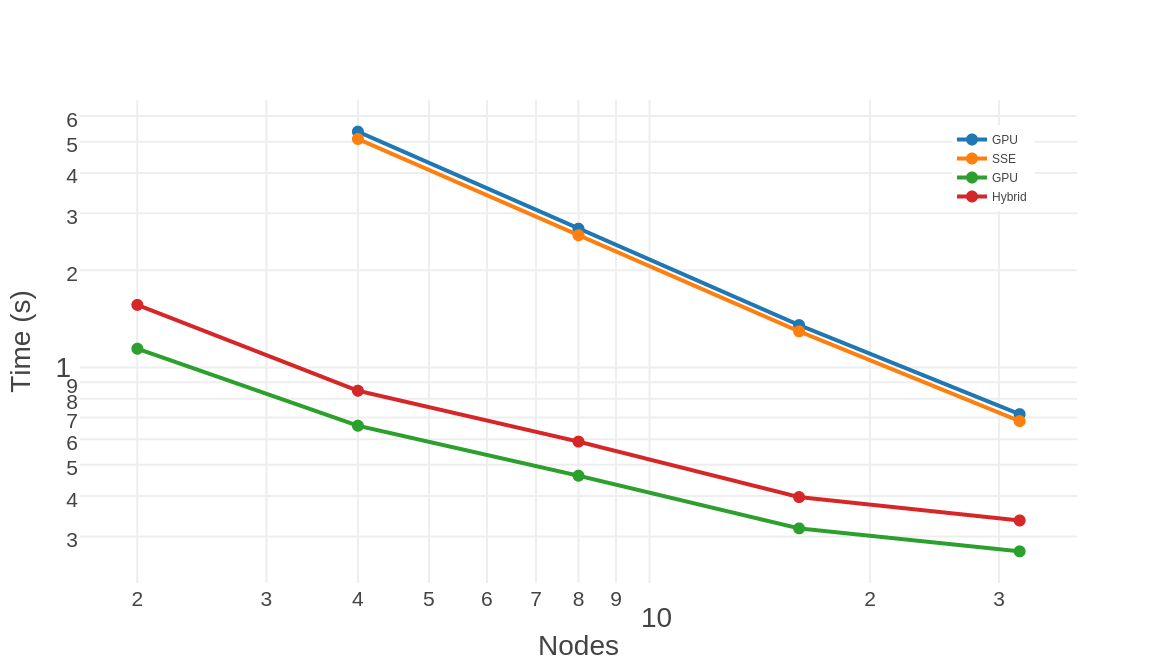
\includegraphics[width=11cm]{Plots/8192.png}
   \caption{Execution time for linear system size: 8192.} \label{plot:bench-8192}

   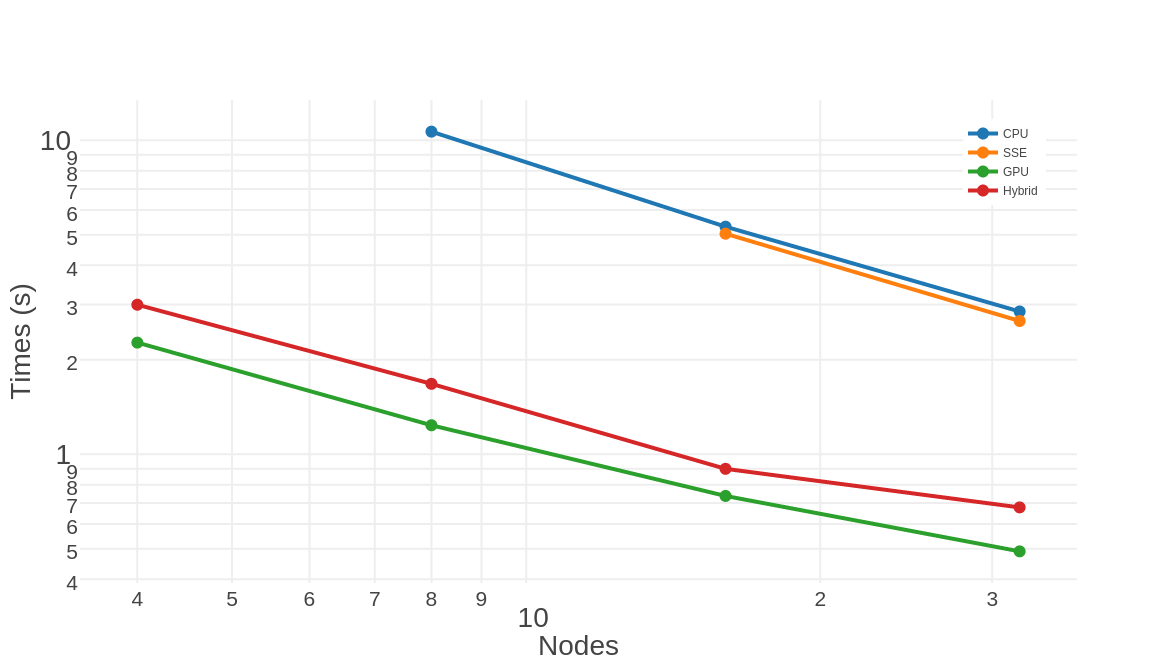
\includegraphics[width=11cm]{Plots/16384.png}
   \caption{Execution time for linear system size: 16384.} \label{plot:bench-16384}
\end{figure}
